\documentclass[14pt]{extbook}
\usepackage{multicol, enumerate, enumitem, hyperref, color, soul, setspace, parskip, fancyhdr} %General Packages
\usepackage{amssymb, amsthm, amsmath, latexsym, units, mathtools} %Math Packages
\everymath{\displaystyle} %All math in Display Style
% Packages with additional options
\usepackage[headsep=0.5cm,headheight=12pt, left=1 in,right= 1 in,top= 1 in,bottom= 1 in]{geometry}
\usepackage[usenames,dvipsnames]{xcolor}
\usepackage{dashrule}  % Package to use the command below to create lines between items
\newcommand{\litem}[1]{\item#1\hspace*{-1cm}\rule{\textwidth}{0.4pt}}
\pagestyle{fancy}
\lhead{Progress Quiz 10}
\chead{}
\rhead{Version A}
\lfoot{5170-5105}
\cfoot{}
\rfoot{Summer C 2021}
\begin{document}

\begin{enumerate}
\litem{
Choose the graph of the equation below.\[ f(x) = \sqrt{x + 6} - 7 \]\begin{enumerate}[label=\Alph*.]
\begin{multicols}{2}\item 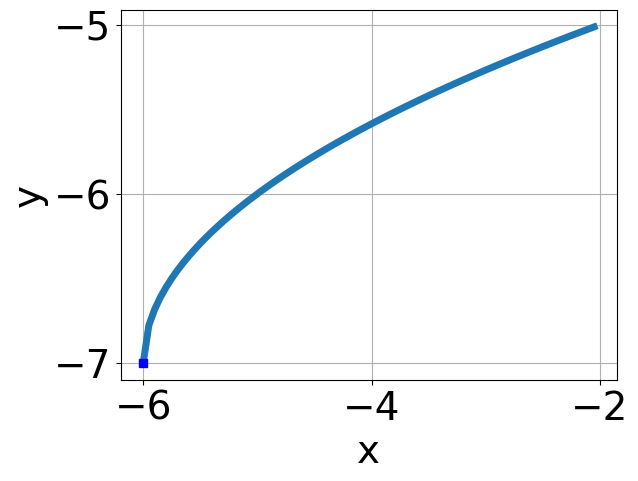
\includegraphics[width = 0.3\textwidth]{../Figures/radicalEquationToGraphAA.png}\item 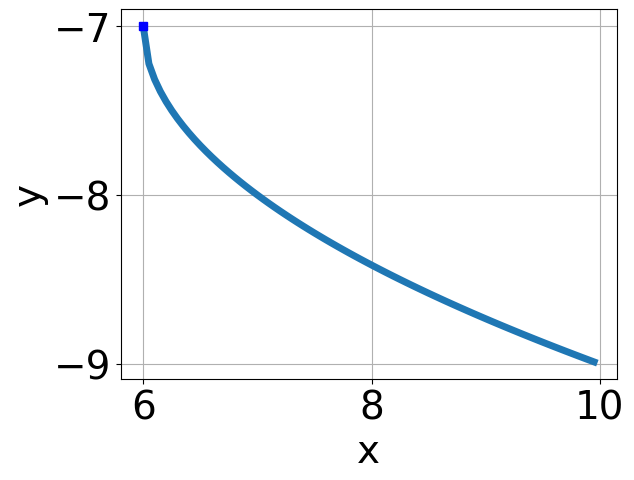
\includegraphics[width = 0.3\textwidth]{../Figures/radicalEquationToGraphBA.png}\item 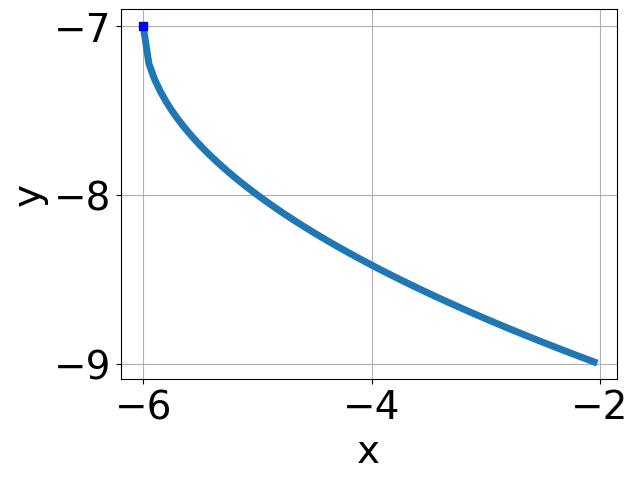
\includegraphics[width = 0.3\textwidth]{../Figures/radicalEquationToGraphCA.png}\item 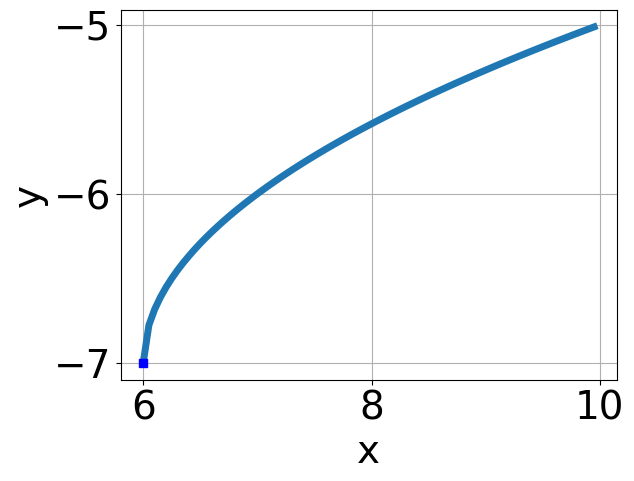
\includegraphics[width = 0.3\textwidth]{../Figures/radicalEquationToGraphDA.png}\end{multicols}\item None of the above.
\end{enumerate} }
\litem{
Solve the radical equation below. Then, choose the interval(s) that the solution(s) belongs to.\[ \sqrt{14 x^2 + 10} - \sqrt{39 x} = 0 \]\begin{enumerate}[label=\Alph*.]
\item \( x \in [-0.2,1.2] \)
\item \( \text{All solutions lead to invalid or complex values in the equation.} \)
\item \( x_1 \in [-0.2, 1.2] \text{ and } x_2 \in [2.5,5.5] \)
\item \( x_1 \in [-4.5, -0.9] \text{ and } x_2 \in [-5.29,0.71] \)
\item \( x \in [1.9,5.3] \)

\end{enumerate} }
\litem{
Choose the equation of the function graphed below.
\begin{center}
    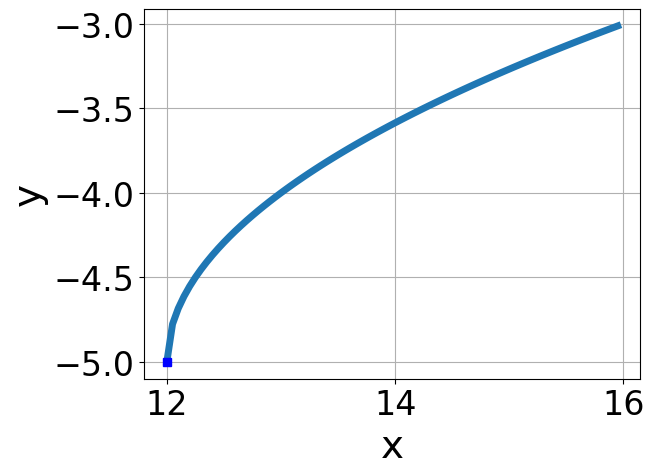
\includegraphics[width=0.5\textwidth]{../Figures/radicalGraphToEquationA.png}
\end{center}
\begin{enumerate}[label=\Alph*.]
\item \( f(x) = \sqrt[3]{x - 12} - 5 \)
\item \( f(x) = - \sqrt[3]{x - 12} - 5 \)
\item \( f(x) = \sqrt[3]{x + 12} - 5 \)
\item \( f(x) = - \sqrt[3]{x + 12} - 5 \)
\item \( \text{None of the above} \)

\end{enumerate} }
\litem{
Choose the graph of the equation below.\[ f(x) = - \sqrt[3]{x + 12} + 6 \]\begin{enumerate}[label=\Alph*.]
\begin{multicols}{2}\item 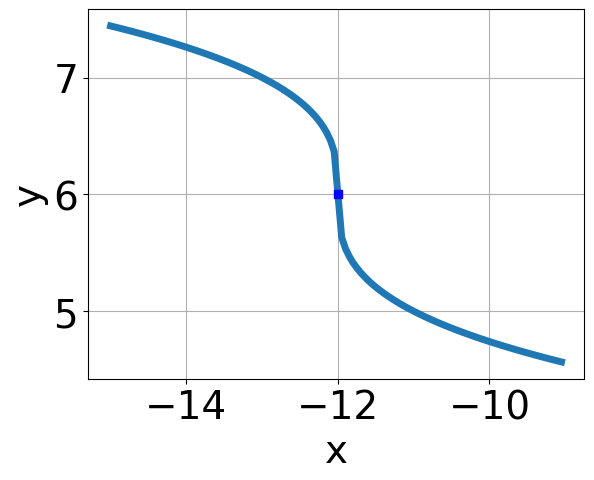
\includegraphics[width = 0.3\textwidth]{../Figures/radicalEquationToGraphCopyAA.png}\item 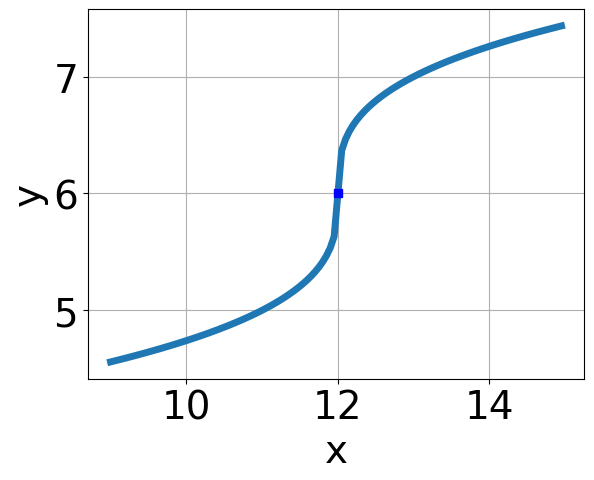
\includegraphics[width = 0.3\textwidth]{../Figures/radicalEquationToGraphCopyBA.png}\item 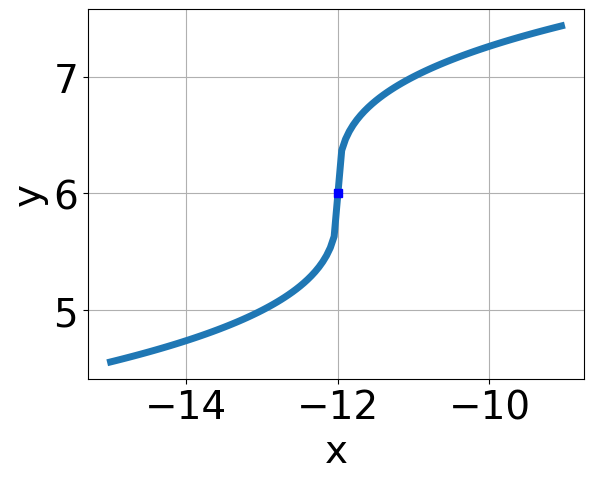
\includegraphics[width = 0.3\textwidth]{../Figures/radicalEquationToGraphCopyCA.png}\item 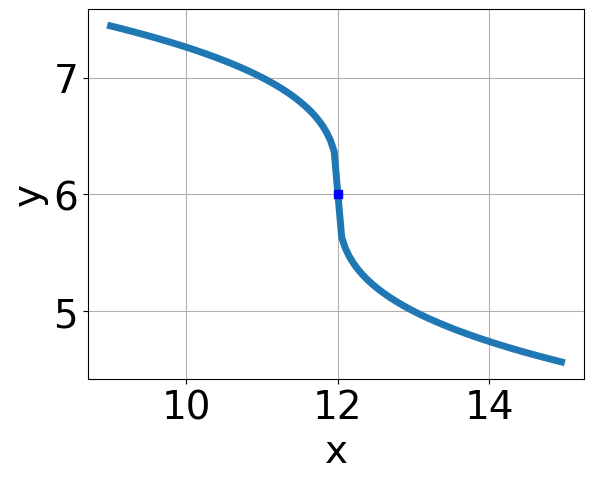
\includegraphics[width = 0.3\textwidth]{../Figures/radicalEquationToGraphCopyDA.png}\end{multicols}\item None of the above.
\end{enumerate} }
\litem{
What is the domain of the function below?\[ f(x) = \sqrt[5]{9 x + 3} \]\begin{enumerate}[label=\Alph*.]
\item \( \text{The domain is } (-\infty, a], \text{   where } a \in [-2.33, 2.67] \)
\item \( (-\infty, \infty) \)
\item \( \text{The domain is } [a, \infty), \text{   where } a \in [-5, -2] \)
\item \( \text{The domain is } [a, \infty), \text{   where } a \in [-2.33, 3.67] \)
\item \( \text{The domain is } (-\infty, a], \text{   where } a \in [-5, -2] \)

\end{enumerate} }
\litem{
Solve the radical equation below. Then, choose the interval(s) that the solution(s) belongs to.\[ \sqrt{2 x + 2} - \sqrt{-4 x - 4} = 0 \]\begin{enumerate}[label=\Alph*.]
\item \( x \in [-0.9,4] \)
\item \( x \in [-2.2,-0.1] \)
\item \( x_1 \in [-2.2, -0.1] \text{ and } x_2 \in [-2,3] \)
\item \( x_1 \in [-2.2, -0.1] \text{ and } x_2 \in [-2,3] \)
\item \( \text{All solutions lead to invalid or complex values in the equation.} \)

\end{enumerate} }
\litem{
Solve the radical equation below. Then, choose the interval(s) that the solution(s) belongs to.\[ \sqrt{2 x - 5} - \sqrt{-5 x - 2} = 0 \]\begin{enumerate}[label=\Alph*.]
\item \( x \in [-0.04,0.7] \)
\item \( x \in [0.86,1.64] \)
\item \( \text{All solutions lead to invalid or complex values in the equation.} \)
\item \( x_1 \in [-0.8, -0.19] \text{ and } x_2 \in [0.5,5.5] \)
\item \( x_1 \in [-0.04, 0.7] \text{ and } x_2 \in [0.5,5.5] \)

\end{enumerate} }
\litem{
What is the domain of the function below?\[ f(x) = \sqrt[4]{-7 x - 4} \]\begin{enumerate}[label=\Alph*.]
\item \( (-\infty, \infty) \)
\item \( (-\infty, a], \text{where } a \in [-4.6, -1.5] \)
\item \( [a, \infty), \text{where } a \in [-5, -0.7] \)
\item \( (-\infty, a], \text{ where } a \in [-0.8, 1.6] \)
\item \( [a, \infty), \text{where } a \in [-0.7, 0.2] \)

\end{enumerate} }
\litem{
Choose the equation of the function graphed below.
\begin{center}
    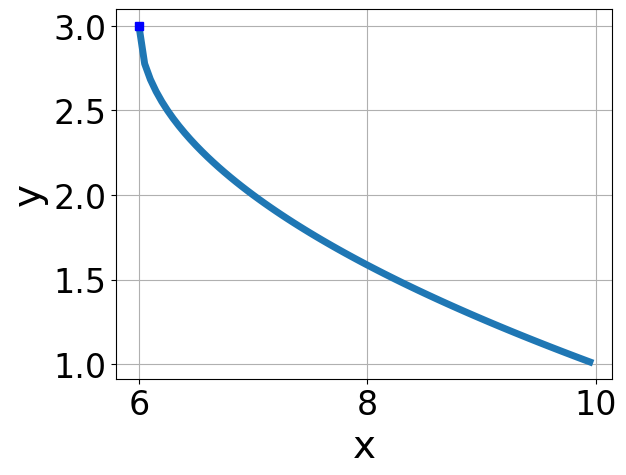
\includegraphics[width=0.5\textwidth]{../Figures/radicalGraphToEquationCopyA.png}
\end{center}
\begin{enumerate}[label=\Alph*.]
\item \( f(x) = - \sqrt{x + 6} + 3 \)
\item \( f(x) = \sqrt{x - 6} + 3 \)
\item \( f(x) = - \sqrt{x - 6} + 3 \)
\item \( f(x) = \sqrt{x + 6} + 3 \)
\item \( \text{None of the above} \)

\end{enumerate} }
\litem{
Solve the radical equation below. Then, choose the interval(s) that the solution(s) belongs to.\[ \sqrt{18 x^2 + 72} - \sqrt{90 x} = 0 \]\begin{enumerate}[label=\Alph*.]
\item \( \text{All solutions lead to invalid or complex values in the equation.} \)
\item \( x \in [-2.3,2.4] \)
\item \( x_1 \in [-2.3, 2.4] \text{ and } x_2 \in [4,8] \)
\item \( x \in [2.4,4.1] \)
\item \( x_1 \in [-5.9, -3.9] \text{ and } x_2 \in [-4,2] \)

\end{enumerate} }
\end{enumerate}

\end{document}